\chapter{Case studies}
To evaluate the effectiveness of the presented frameworks, we use three case studies. In each case
study, we benchmark the frameworks using the following steps:
\begin{enumerate}
    \item Describe the system of concern.
    \item Construct parametric DTMC models and formalize a property of interest for parameter synthesis.
    \item Select model true parameters arbitrarily random and generate synthetic data from it.
    \item Apply the frameworks for both rational functions and simulation-based setups.
    \item Visualize the parameter synthesis and inference result.
    \item Measure runtime among different model sizes.
    \item Discussion on results.
\end{enumerate}
The first case study is \textit{IPv4 ZeroConfiguration Protocol}. The second case study comes from
the experiments of the Department of Biology at the University of Konstanz on the defensive
behaviour of bee colonies\cite{hajnal2019data}. The third case study is a stochastic SIR model of
epidemics; it is introduced in order to show the expansion of the model state-space as the system
has more states to be encoded. All experiments are conducted in the following system:
\begin{itemize}
    \item Intel Xeon W-2135 processor, 64GB RAM, OpenSUSE 15.2
    \item Python 3.8.8, StormPy 1.6.3, Storm stable, PRISM 4.6
\end{itemize}

%%%%%%%%%%%%%%%%%%%%%%%%%%%%%%%%%%%%%%%%%%%%%%%%%%%%%%%%%%%%%%%%%%%%%%%%%%%%%%%%%%%%%%%%%%%%%%%%%%%

\section{ZeroConfiguration Protocol}
\subsection{System description}
Zero-configuration protocol (\textit{zeroconf} for short) \cite{ZeroConf} is a protocol used in IPv4 network to
allocate newly attached device an unique IP address without any intervention from network operators.
\begin{algorithm}[H]
    \caption{IPv4 Zeroconf procedure.}
    \label{alg:gen-sir-ctmc}
    \footnotesize{
        \hspace*{\algorithmicindent} \textbf{Input:} $N$: number of probes.\\
        \hspace*{\algorithmicindent} \textbf{Output:} An unused address, or abort with error.
    }
    \begin{algorithmic}[1]
        \Procedure{Zeroconf}{}
        \State Select an address $ip$ randomly
        \State $i = 1$
        \While{$i \leq N$}
        \State Broadcast message asking if $ip$ is already in use.
        \If{Received reply that $ip$ is in use}
        \State Select an address $ip$ randomly
        \State Continue loop.
        \EndIf
        \If{timeout}
        \If{$i = N$}
        \State Return $ip$
        \EndIf
        \State $i \leftarrow i + 1$
        \State Continue loop.
        \EndIf
        \EndWhile
        \EndProcedure
    \end{algorithmic}
\end{algorithm}

\subsection{Model and properties}
We introduce two real parameters $(p, q) \in [0,1]\times[0,1]$.
\begin{itemize}
    \item $p$: probability of a message is loss (no reply and timed out).
    \item $q$: received a reply that $ip$ is in use.
\end{itemize}
By replace non-determinisms (timeout and address occupied) by probability distribution, we construct
the a parametric DTMC as a formalism of the Zeroconf protocol of $N$ probes.
\begin{figure}[H]
    \centering
    \begin{tikzpicture}[->, >=stealth', auto, semithick, node distance=2.5cm]
        \tikzstyle{every state}=[font=\footnotesize, fill=white,draw=black,thick,text=black,scale=1]
        \node[state, initial]    (A)            {$S_0$};
        \node[state]    (B)[below of=A]         {};
        \node[state,accepting]    (I)[below of=B]         {$\text{OK}$};

        \node[state]    (C)[right of=A]         {$S_1$};
        \node[state]    (D)[right of=C]         {$S_2$};
        \node[state]    (E)[right of=D]         {$S_3$};
        \node[state]    (F)[right of=E]         {$S_4$};
        \node[state]    (G)[below of=F]         {};
        \node[state,accepting]    (H)[below of=G]         {$\text{Failed}$};

        \path
        (A)
        edge    node{$q$}       (C)
        edge    node[left]{$1-q$}     (B)

        (B)
        edge    node[left]{$1$}     (I)

        (I)
        edge [loop below] node{$1$} (I)

        (C)
        edge    node{$p$}          (D)
        edge [bend left] node{$1-p$}        (A)

        (D)
        edge    node{$p$}          (E)
        edge  [bend left=50]  node{$1-p$}        (A)

        (E)
        edge    node{$p$}          (F)
        edge  [bend left=60]  node{$1-p$}        (A)

        (F)
        edge    node{$p$}          (G)
        edge [bend left=70]  node{$1-p$}        (A)

        (G)
        edge    node{$1$}          (H)

        (H)
        edge [loop below] node{$1$} (G);

    \end{tikzpicture}
    \label{fig:zeroconf-4}
    \caption{Example of an IPv4 Zeroconf model with 4 probes}
\end{figure}
\noindent We want to verify the following property: \textit{"Eventually, an IP is successfully
    allocated with at most $N$ probes with probability of at least 75 percents."} In PCTL formula
\begin{align*}
    P_{\geq 0.75} ( \texttt{true} \quad \mathsf{U}^{\leq N} \quad \texttt{"OK"} )
\end{align*}

\subsection{Evaluation}
\subsubsection{True parameters and synthetic data}
We select a true parameter $(p, q)$ arbitrarily random.
\begin{table}[H]
    \begin{tabular}{|l|l|l|}
        \hline
        Model $\mathcal{M}$           & Zeroconf, 4 probes                                                  & Zeroconf, 10 probes                                                  \\ \hline
        Number of BSCCs               & 2                                                                   & 2                                                                    \\ \hline
        Number of states              & 9                                                                   & 14                                                                   \\ \hline
        True parameter $\theta=(p,q)$ & (0.105547, 0.449658)                                                & (0.197779, 0.621824)                                                 \\ \hline
        Number of samples             & 10000                                                               & 10000                                                                \\ \hline
        Synthetic data $D_{obs}$      & (41, 9959)                                                          & (22, 9978)                                                           \\ \hline
        Property of interest $\Phi$   & $P_{\geq 0.75} (\texttt{true} \mathsf{U}^{\leq 4} (\texttt{"OK"}))$ & $P_{\geq 0.75} (\texttt{true} \mathsf{U}^{\leq 10} (\texttt{"OK"}))$ \\ \hline
        \begin{tabular}[c]{@{}l@{}}Satisfaction property\\ $P(\mathcal{M}_\theta\models\Phi)$\end{tabular}     & 0.946409                                                            & 0.952067                                                             \\ \hline
    \end{tabular}
    \caption{Synthetic data for Zeroconf model of 4 and 10 probes.}
\end{table}


\subsubsection{Parameter synthesis results}
In the following parameter synthesis experiment, we set the number of samples in Sequential Monte
Carlo $N=200$ and the number of perturbation kernels $M=19$. Perturbation and transition kernel are
selected as described in Chapter 4. In RF-SMC, the length of Metropolis-Hasting is $N_{MH}=50$. In
SMC-ABC-SMC, the distance threshold is $\epsilon=0.25$.\\
First, we present the parameter synthesis result for Zeroconf parametric DTMC of 4 probes. The
property of interest is
\begin{align*}
    P_{\geq 0.75} (\texttt{true} \mathsf{U}^{\leq 4} (\texttt{"OK"}))
\end{align*}
\begin{table}[H]
    \begin{tabular}{|l|l|l|}
        \hline
        Method                                           & RF-SMC               & SMC-ABC-SMC          \\ \hline
        Estimated parameter $\hat{\theta}$               & (0.188956, 0.460554) & (0.176469, 0.355322) \\ \hline
        True parameter $\theta$                          & (0.105547, 0.449658) & (0.105547, 0.449658) \\ \hline
        L2 distance $\Vert \theta, \hat{\theta} \Vert_2$ & 0.084117             & 0.118023             \\ \hline
        $P(\mathcal{M}_{\hat{\theta}}\models\Phi)$       & 0.893715             & 0.918133             \\ \hline
    \end{tabular}
    \caption{Parameter estimation results for Zeroconf model of 4 probes.}
\end{table}

\begin{figure}[H]
    \centering
    \begin{subfigure}{0.48\textwidth}
        \centering
        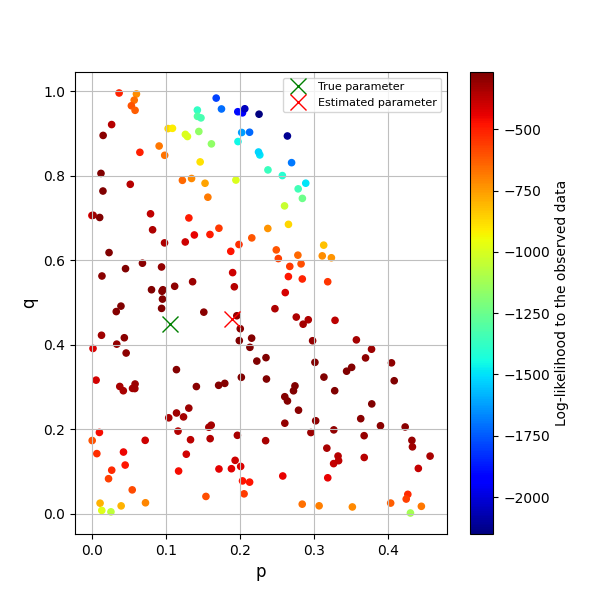
\includegraphics[width=\linewidth]{figures/zeroconf4_rf.png}
        \caption{Sampled particles using Rational Functions SMC}
    \end{subfigure}
    \hfill
    \begin{subfigure}{0.48\textwidth}
        \centering
        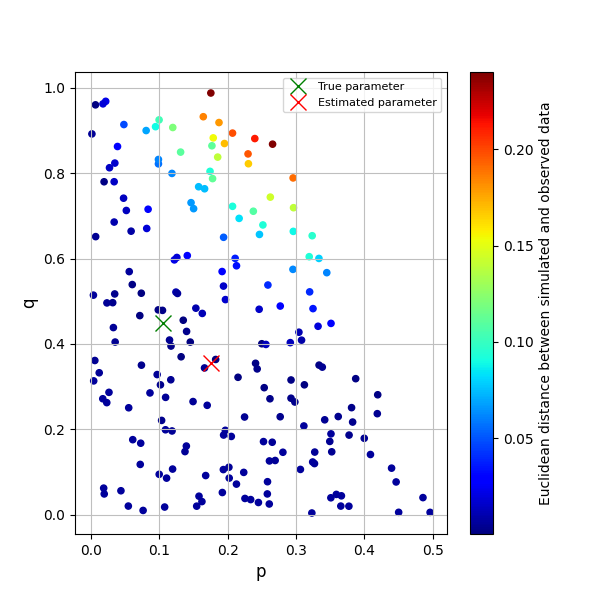
\includegraphics[width=\linewidth]{figures/zeroconf4_sim.png}
        \caption{Sampled particles using Statiscal Model Checking ABC-SMC}
    \end{subfigure}
    \caption{Parameter synthesis results for Zeroconf model of 4 probes.}
\end{figure}

\newpage
\noindent We present parameter synthesis results for Zeroconf parametric DTMC of 10 probes. We use
the same RF-SMC and SMC-ABC-SMC framework configuration as in the parameter synthesis of the
Zeroconf model with four probes.
\begin{align*}
    P_{\geq 0.75} (\texttt{true} \mathsf{U}^{\leq 10} (\texttt{"OK"}))
\end{align*}
\begin{table}[H]
    \begin{tabular}{|l|l|l|}
        \hline
        Method                                           & RF-SMC               & SMC-ABC-SMC          \\ \hline
        True parameter $\theta$                          & (0.197779, 0.621824) & (0.197779, 0.621824) \\ \hline
        Estimated parameter $\hat{\theta}$               & (0.301807, 0.457090) & (0.378774, 0.405870) \\ \hline
        L2 distance $\Vert \theta, \hat{\theta} \Vert_2$ & 0.194831             & 0.281772             \\ \hline
        $P(\mathcal{M}_{\hat{\theta}}\models\Phi)$       & 0.952067             & 0.966142             \\ \hline
    \end{tabular}
    \caption{Parameter estimation results for Zeroconf model of 10 probes.}
\end{table}

\begin{figure}[H]
    \centering
    \begin{subfigure}{0.48\textwidth}
        \centering
        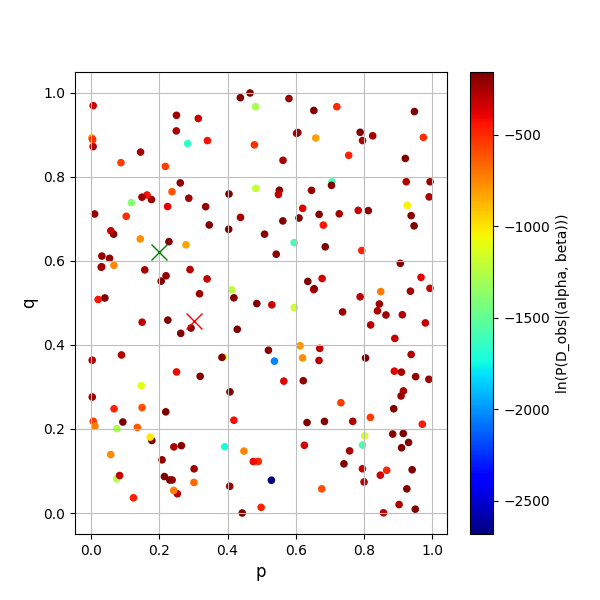
\includegraphics[width=\linewidth]{figures/zeroconf10_rf.png}
        \caption{Sampled particles using RF-SMC}
    \end{subfigure}
    \hfill
    \begin{subfigure}{0.48\textwidth}
        \centering
        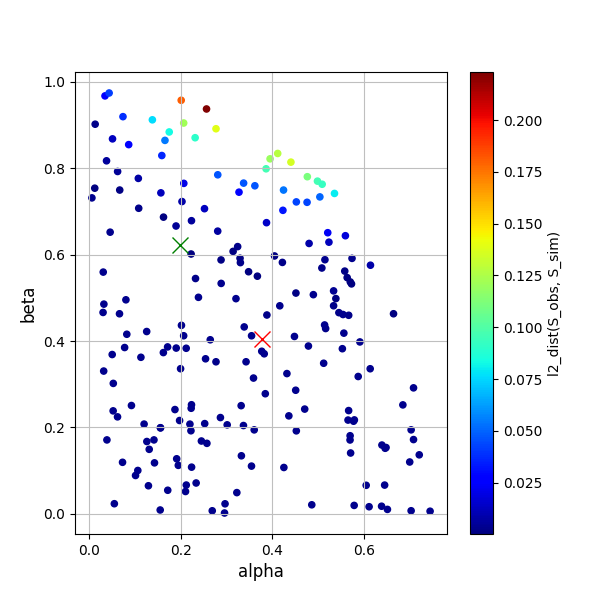
\includegraphics[width=\linewidth]{figures/zeroconf10_sim.png}
        \caption{Sampled particles using SMC-ABC-SMC}
    \end{subfigure}
    \caption{Parameter synthesis results for Zeroconf model of 10 probes.}
\end{figure}

\subsection{Performance}
To measure the performance of RF-SMC and SMC-ABC-SMC, we measure the physical runtime to finish
\textit{(total runtime)} and the average physical run time of one perturbation kernel
\textit{(average perturbation runtime)}.
\begin{table}[H]
    \centering
    \begin{tabular}{|l|l|l|}
        \hline
        Method                     & RF-SMC & SMC-ABC-SMC \\ \hline
        Total runtime (minutes)    & 6.083  & 54.867      \\ \hline
        \begin{tabular}[c]{@{}l@{}}Average perturbation\\ runtime (minutes)\end{tabular} & 0.32   & 2.88        \\ \hline
    \end{tabular}
    \caption{Physical runtime on Zeroconf model with 4 probes.}
\end{table}
\begin{table}[H]
    \centering
    \begin{tabular}{|l|l|l|}
        \hline
        Method                     & RF-SMC & SMC-ABC-SMC \\ \hline
        Total runtime (minutes)    & 9.50   & 37.93       \\ \hline
        \begin{tabular}[c]{@{}l@{}}Average perturbation\\ runtime (minutes)\end{tabular} & 0.501  & 1.978       \\ \hline
    \end{tabular}
    \caption{Physical runtime on Zeroconf model with 10 probes.}
\end{table}
\begin{figure}[H]
    \centering
    \begin{subfigure}{0.48\textwidth}
        \centering
        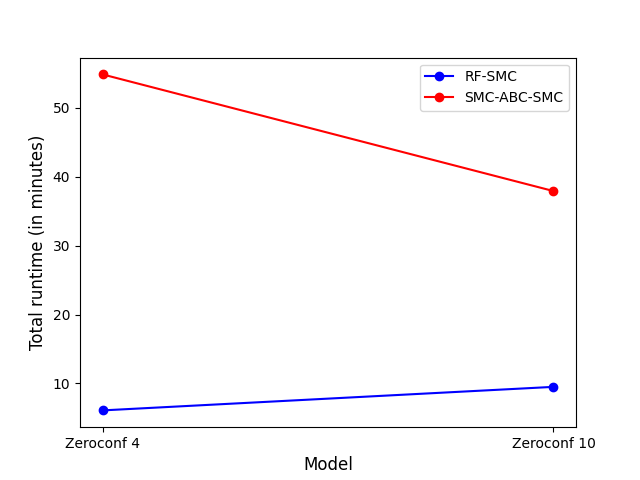
\includegraphics[width=\linewidth]{figures/zeroconf_runtime_total.png}
        \caption{Total runtime}
    \end{subfigure}
    \hfill
    \begin{subfigure}{0.48\textwidth}
        \centering
        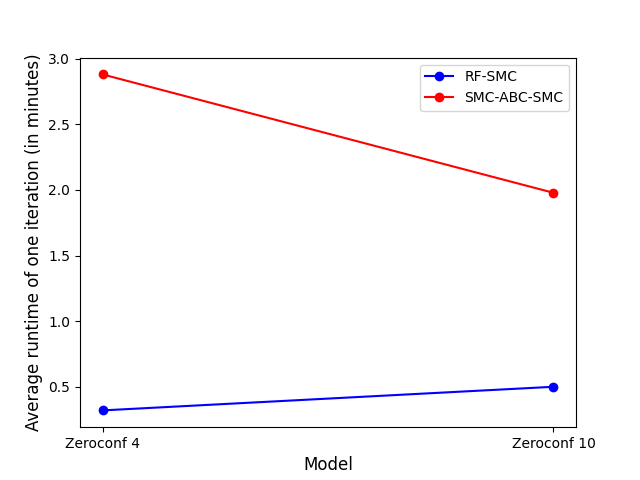
\includegraphics[width=\linewidth]{figures/zeroconf_runtime_avg.png}
        \caption{Average perturbation runtime}
    \end{subfigure}
    \caption{Physical runtime on Zeroconf model of different sizes.}
\end{figure}

\subsection{Discussion}
In the experiments with Zeroconf models of 4 and 10 probes, RF-SMC and ABC-SMC have comparable
accuracy in parameter estimation. The parameter synthesis results suggest that parameter accepting
region and rejecting region are linearly separated in the first quadrant of the 2D Cartesian plane.
In terms of performance, rational function evaluation is faster than simulation in the two models.
However, the performance gap is narrower in the 10-probes model. It suggests that the
simulation-based method is probably preferable for Zeroconf models with more probes in terms of
performance. In the next experiment with models of honey bees colony, we investigate the accuracy
and performance of the rational function-based method and simulation-based method with models of
more complicated transitions.

%%%%%%%%%%%%%%%%%%%%%%%%%%%%%%%%%%%%%%%%%%%%%%%%%%%%%%%%%%%%%%%%%%%%%%%%%%%%%%%%%%%%%%%%%%%%%%%%%%%
\section{Social feedback in honeybee colonies}
\subsection{System description}
We study the collective behavior of a bee colony. Each bee in a colony possibly stings after
observing a threat in the surrounding environment and warns other bees by releasing a special
substance, pheromone. By sensing the pheromone released in the environment, other bees in the colony
may also sting. Assume that each bee in a colony decides its following action (to sting or not to
sting) based only on the current state of the environment; we model the number of bees who sting or
not sting by Markov population processes. To reduce the complexity of the model, we make another
assumption that the states of the bee colony are observed after a uniform time duration. Hence the
model is of discrete-time. However, since stinging leads to the termination of an individual bee, it
reduces the total defense capability.

\subsection{Model and properties}
With the parametric Discrete-time Markov chain as the model, we study how a single bee's actions
change regarding the colony size and pheromone amount. There are 3 assumptions on the system:
\begin{enumerate}
    \item Each bee releases a unit amount of pheromone immediately after stinging.
    \item A bee dies after stinging and releasing a pheromone unit. In other words, no bee can sting
          more than once.
    \item Stinging behavior only depends on the concentration of pheromone in the environment.
\end{enumerate}
Under these assumptions, a bee colony can be viewed as a set of agents (bees) that interact with
each other in a closed environment with the appearance of a factor \textit{pheromone}. Afterward,
the agent has a probability of committing an action, namely \textit{sting}. The agent is eliminated
from the environment after stinging. Assume that we have a colony of $n$ bees initially. As
aforementioned, an individual bee dies after it stings. Thus, at the end of the experiment, the number
of bees is $n'\in\{0,1,\ldots,n\}$. We model the bee colony with a DTMC $\mathcal{M}=(S,\mathbf{P},
    S_{init}, AP,L)$, such that
\begin{itemize}
    \item $|S_{init}|=1$
    \item There exists $n+1$ BSCCs which encode the population at the end of the experiment.
\end{itemize}
Semantics of Markov population models for bees colony are developed by \cite{hajnal2019data}.
\begin{example}{Parametric DTMC model of 3 bees.}
    We model a colony of 3 bees using parametric DTMC. In the following DTMC model, each individual
    bee is encode by an integer represents its state
    \begin{itemize}
        \item $0$: bee never stings.
        \item $1$: bee stings and dies.
        \item $2$: bee does not sting in $2$ consecutive observations.
        \item $k$: bee does not sting in $k$ consecutive observations.
    \end{itemize}
    Let $p, q_1, q_2$ represent the probabilities that a bee stings without any stimulation and a
    bee stings at 1 and 2 attemps, respectively. We then construct the following parametric DTMC
    \begin{figure}[H]
        \centering
        \begin{tikzpicture}[->, >=stealth', auto, semithick, node distance=3cm, font=\footnotesize]
            \tikzstyle{every state}=[font=\footnotesize , fill=white,draw=black,thick,text=black,scale=1]
            \node[state,initial]    (A)                     {init};
            \node[state]            (B)[right of=A]         {$2, 2, 1 $};
            \node[state,accepting]  (C)[above of=B]         {$0, 0, 0$};
            \node[state]            (D)[below of=B]         {$2, 1, 1$};
            \node[state,accepting]  (E)[below of=A]         {$1, 1, 1$};
            \node[state]            (F)[right of=B]         {$0, 2, 1$};
            \node[state,accepting]  (G)[right of=D]         {$0, 1, 1$};
            \node[state,accepting]  (H)[right of=F]         {$0, 0, 1$};
            \path
            (A)
            edge    node{$3p(1-p)^2$}      (B)
            edge    node{$(1-p)^3$}        (C)
            edge    node{$3p(1-p)^2$}      (D)
            edge    node{$p^3$}            (E)
            (B)
            edge    node{$1-q_1$}            (F)
            edge    node{$q_1$}              (D)

            (C)
            edge [loop right] node {1} (C)

            (D)
            edge    node{$1-q_2$}          (G)
            edge    node{$q_2$}              (E)
            (E)
            edge [loop left] node {1} (W)
            (F)
            edge    node{$q_1$}              (G)
            edge    node{$1 - q_1$}          (H)
            (G)
            edge [loop right] node {1} (G);
        \end{tikzpicture}
        \caption{Parametric DTMC model of 3 bees with 3 parameters $p, q_1, q_2$}
    \end{figure}
\end{example}
In studying the defensive behaviors of bee colonies regarding social feedback, we are interested in
the number of stimulated bees who decide to sting. Therefore, we verify the following property:
\textit{"With a probability of at least 25 percent, at least a half of bees population survives."}
In PCTL formula:
\begin{align*}
    P_{\geq 0.25} ( \texttt{true} \quad \mathsf{U} \quad \texttt{"|Survived| > 0.5N"} )
\end{align*}

\subsection{Evaluation}
\subsubsection{True parameters and synthetic data}
We select arbitrary true parameters to generate synthetic data and obtain steady-state distribution.
Let $S$ be the number of survived bees at the steady-state. We sample DTMCs instantiated from true
parameters $10000$ times to obtain steady-state distribution.
\begin{table}[H]
    \footnotesize
    \centering
    \begin{tabular}{|l|l|l|l|}
        \hline
        Model $\mathcal{M}$                & 3 bees                                         & 5 bees                                           & 10 bees                                          \\ \hline
        Number of states                   & 13                                             & 24                                               & 69                                               \\ \hline
        Number of BSCCs                    & 4                                              & 6                                                & 11                                               \\ \hline
        True parameter $\theta$            & \begin{tabular}[c]{@{}l@{}}$p=0.665623$ \\ $q_1=0.830401$ \\ $q_2=0.839778$ \end{tabular}                     & \begin{tabular}[c]{@{}l@{}}$p=0.278370$ \\ $q_1=0.305994$ \\ $q_2=0.489792$ \\ $q_3=0.737252$ \\ $q_4=0.766581$ \end{tabular}                       & \begin{tabular}[c]{@{}l@{}}$p=0.222169$ \\ $q_1=0.246993$ \\ $q_2=0.281934$ \\ $q_3=0.446384$ \\ $q_4=0.491612$ \\ $q_5=0.534611$ \\ $q_6=0.569409$ \\ $q_7=0.684651$ \\ $q_8=0.717139$ \\ $q_9=0.800987$  \end{tabular}                       \\ \hline
        Synthetic data $D_{obs}$           & (344, 54, 1390, 8212)                          & \begin{tabular}[c]{@{}l@{}}(1940, 11, 216, \\ 2682, 4200, 951)\end{tabular}                       & \begin{tabular}[c]{@{}l@{}}(769, 0, 1, 10, 187, 972,\\  2494, 2982, 2133, 419, 33)\end{tabular}                       \\ \hline
        Property of interest $\Phi$        & $P_{\geq 0.25} (\text{true} \mathsf{U} (S>3))$ & $P_{\geq 0.25} (\texttt{true} \mathsf{U} (S>5))$ & $P_{\geq 0.25} (\texttt{true} \mathsf{U} (S>8))$ \\ \hline
        $P(\mathcal{M}_\theta\models\Phi)$ & 0.819666                                       & 0.780172                                         & 0.737244                                         \\ \hline
    \end{tabular}
    \caption{True parameter and synthetic data for 3, 5, and 10 bees models.}
\end{table}
\begin{figure}[H]
    \centering
    \begin{subfigure}{0.32\textwidth}
        \centering
        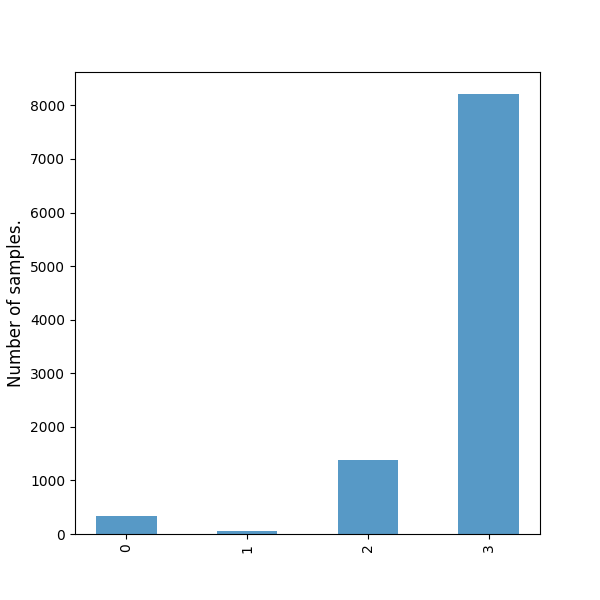
\includegraphics[width=\linewidth]{figures/bee_3_data.png}
        \caption{3 bees model.}
    \end{subfigure}
    \hfill
    \begin{subfigure}{0.32\textwidth}
        \centering
        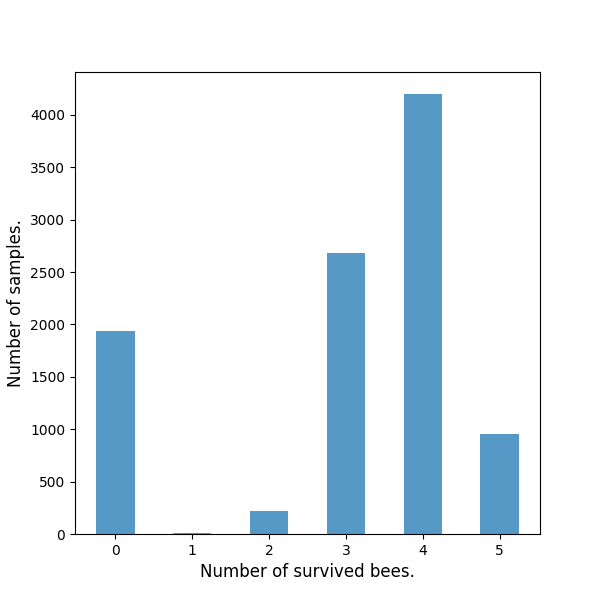
\includegraphics[width=\linewidth]{figures/bee_5_data.png}
        \caption{5 bees model.}
    \end{subfigure}
    \hfill
    \begin{subfigure}{0.32\textwidth}
        \centering
        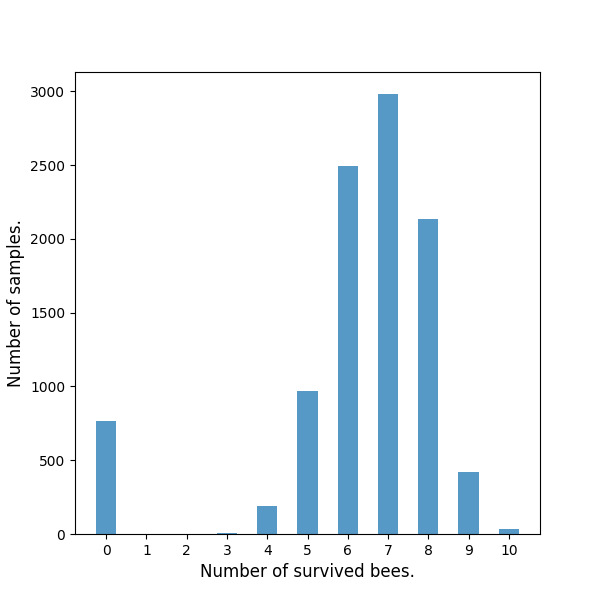
\includegraphics[width=\linewidth]{figures/bee_10_data.png}
        \caption{10 bees model.}
    \end{subfigure}
    \caption{Histogram of steady-state data obtained from $10000$ simulation runs.}
\end{figure}

\subsubsection{Parameter synthesis results}
We set the number of samples in Sequential Monte Carlo $N=200$ and the number of perturbation
kernels $M=19$. In RF-SMC, the length of Metropolis-Hasting is $N_{MH}=50$. In SMC-ABC-SMC, the
distance threshold is $\epsilon=0.25$. Perturbation and transition kernels are component-wise
uniform distribution. Prior distribution is $Uniform(0,1)$.\\
Parameter synthesis results for 3, 5, and 10 bees model:
\begin{table}[H]
    \centering
    \begin{tabular}{|l|l|l|}
        \hline
                                                          & RF-SMC                     & SMC-ABC-SMC                \\ \hline
        True parameter $\theta$                           & \begin{tabular}[c]{@{}l@{}}$p=0.665623$ \\ $q_1=0.830401$ \\ $q_2=0.839778$ \end{tabular} & \begin{tabular}[c]{@{}l@{}}$p=0.665623$ \\ $q_1=0.830401$ \\ $q_2=0.839778$ \end{tabular} \\ \hline
        Estimated parameter $\hat{\theta}$                & \begin{tabular}[c]{@{}l@{}}$p=0.671388$ \\ $q_1=0.575026$ \\ $q_2=0.525502$ \end{tabular} & \begin{tabular}[c]{@{}l@{}}$p=0.811651$ \\ $q_1=0.621073$ \\ $q_2=0.544130$ \end{tabular} \\ \hline
        L2 distance  $\Vert \theta, \hat{\theta} \Vert_2$ & 0.404992                   & 0.390576                   \\ \hline
        $P(\mathcal{M}_{\hat{\theta}}\models\Phi)$        & 0.623889                   & 0.595083                   \\ \hline
    \end{tabular}
    \caption{Parameter synthesis result for 3 bees model.}
\end{table}

\begin{table}[H]
    \centering
    \footnotesize
    \begin{tabular}{|l|l|l|}
        \hline
                                                          & RF-SMC                     & SMC-ABC-SMC                \\ \hline
        True parameter $\theta$                           & \begin{tabular}[c]{@{}l@{}}$p=0.278370$ \\ $q_1=0.305994$ \\ $q_2=0.489792$ \\ $q_3=0.737252$ \\ $q_4=0.766581$ \end{tabular} & \begin{tabular}[c]{@{}l@{}}$p=0.278370$ \\ $q_1=0.305994$ \\ $q_2=0.489792$ \\ $q_3=0.737252$ \\ $q_4=0.766581$ \end{tabular} \\ \hline
        Estimated parameter $\hat{\theta}$                & \begin{tabular}[c]{@{}l@{}}$p=0.576565$ \\ $q_1=0.589724$ \\ $q_2=0.490334$ \\ $q_3=0.554397$ \\ $q_4=0.524433$ \end{tabular} & \begin{tabular}[c]{@{}l@{}}$p=0.361220$ \\ $q_1=0.316007$ \\ $q_2=0.545691$ \\ $q_3=0.643962$ \\ $q_4=0.591206$ \end{tabular} \\ \hline
        L2 distance  $\Vert \theta, \hat{\theta} \Vert_2$ & 0.511366                   & 0.222594                   \\ \hline
        $P(\mathcal{M}_{\hat{\theta}}\models\Phi)$        & 0.623889                   & 0.595083                   \\ \hline
    \end{tabular}
    \caption{Parameter synthesis result for 5 bees model}
\end{table}

\begin{table}[H]
    \centering
    \footnotesize
    \begin{tabular}{|l|l|l|}
        \hline
                                                          & RF-SMC                     & SMC-ABC-SMC                \\ \hline
        True parameter $\theta$                           & \begin{tabular}[c]{@{}l@{}}$p=0.222169$ \\ $q_1=0.246993$ \\ $q_2=0.281934$ \\ $q_3=0.446384$ \\ $q_4=0.491612$ \\ $q_5=0.534611$ \\ $q_6=0.569409$ \\ $q_7=0.684651$ \\ $q_8=0.717139$ \\ $q_9=0.800987$  \end{tabular} & \begin{tabular}[c]{@{}l@{}}$p=0.222169$ \\ $q_1=0.246993$ \\ $q_2=0.281934$ \\ $q_3=0.446384$ \\ $q_4=0.491612$ \\ $q_5=0.534611$ \\ $q_6=0.569409$ \\ $q_7=0.684651$ \\ $q_8=0.717139$ \\ $q_9=0.800987$  \end{tabular} \\ \hline
        Estimated parameter $\hat{\theta}$                & \begin{tabular}[c]{@{}l@{}}$p=0.604881$ \\ $q_1=0.472557$ \\ $q_2=0.281484$ \\ $q_3=0.500706$ \\ $q_4=0.49340$ \\ $q_5=0.495508$ \\ $q_6=0.466596$ \\ $q_7=0.510167$ \\ $q_8=0.474153$ \\ $q_9=0.484061$  \end{tabular} & \begin{tabular}[c]{@{}l@{}}$p=0.391313$ \\ $q_1=0.485688$ \\ $q_2=0.424056$ \\ $q_3=0.381489$ \\ $q_4=0.440681$ \\ $q_5=0.578865$ \\ $q_6=0.594232$ \\ $q_7=0.564557$ \\ $q_8=0.547804$ \\ $q_9=0.520006$  \end{tabular} \\ \hline
        L2 distance  $\Vert \theta, \hat{\theta} \Vert_2$ & 0.665837                   & 0.487042                   \\ \hline
        $P(\mathcal{M}_{\hat{\theta}}\models\Phi)$        & 0.933287                   & 0.907478                   \\ \hline
    \end{tabular}
    \caption{Parameter synthesis result for 10 bees model}
\end{table}

\subsection{Performance}
To measure the performance of RF-SMC and SMC-ABC-SMC, we measure the physical runtime to finish
\textit{(total runtime)} an the average physical run time of one perturbation kernel
\textit{(average perturbation runtime)}.
\begin{table}[H]
    \centering
    \footnotesize
    \begin{tabular}{|l|l|l|}
        \hline
        Method                     & RF-SMC & SMC-ABC-SMC \\ \hline
        Total runtime (minutes)    & 5.917  & 68.783      \\ \hline
        \begin{tabular}[c]{@{}l@{}}Average perturbation\\ runtime (minutes)\end{tabular} & 0.312  & 3.614       \\ \hline
    \end{tabular}
    \caption{Physical runtime on 3 bees model.}
\end{table}
\begin{table}[H]
    \centering
    \footnotesize
    \begin{tabular}{|l|l|l|}
        \hline
        Method                     & RF-SMC & SMC-ABC-SMC \\ \hline
        Total runtime (minutes)    & 29.517 & 352.083     \\ \hline
        \begin{tabular}[c]{@{}l@{}}Average perturbation\\ runtime (minutes)\end{tabular} & 1.553  & 18.518      \\ \hline
    \end{tabular}
    \caption{Physical runtime on 5 bees model.}
\end{table}
\begin{table}[H]
    \centering
    \footnotesize
    \begin{tabular}{|l|l|l|}
        \hline
        Method                     & RF-SMC   & SMC-ABC-SMC \\ \hline
        Total runtime (minutes)    & 3976.117 & 581.833     \\ \hline
        \begin{tabular}[c]{@{}l@{}}Average perturbation\\ runtime (minutes)\end{tabular} & 209.237  & 30.592      \\ \hline
    \end{tabular}
    \caption{Physical runtime on 10 bees model.}
\end{table}
\begin{figure}[H]
    \centering
    \begin{subfigure}{0.4\textwidth}
        \centering
        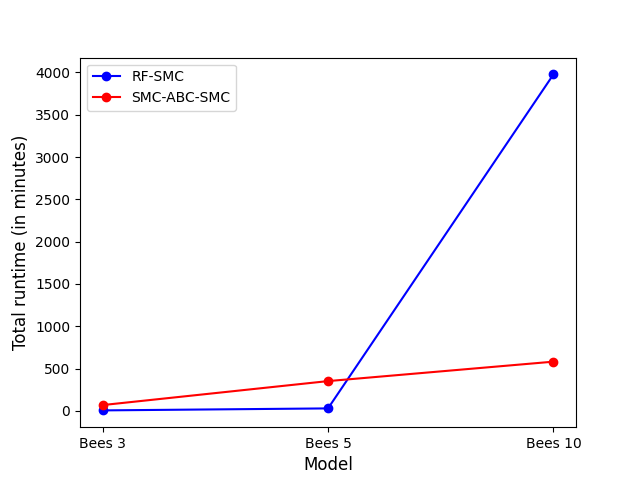
\includegraphics[width=\linewidth]{figures/bees_runtime_total.png}
        \caption{Total runtime}
    \end{subfigure}
    \hfill
    \begin{subfigure}{0.4\textwidth}
        \centering
        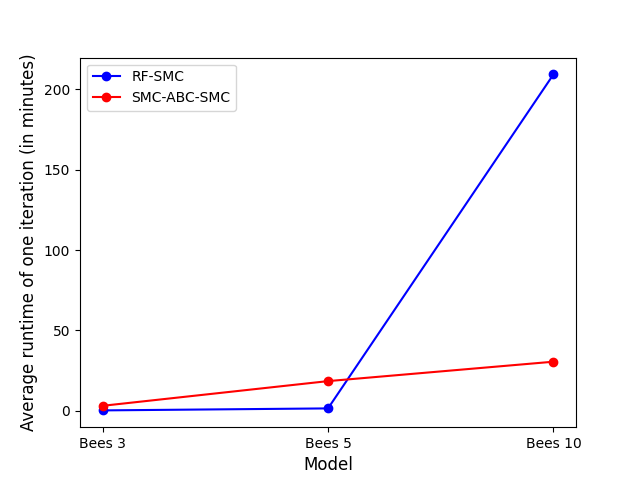
\includegraphics[width=\linewidth]{figures/bees_runtime_avg.png}
        \caption{Average perturbation runtime}
    \end{subfigure}
    \caption{Physical runtime on Zeroconf model of different sizes.}
\end{figure}
\subsection{Discussion}
The case study with bee colony observed that overall, the simulation-based method delivers
estimations that are closer to the true parameter than rational-function-based frameworks. In the
experiments with 3 bees and 5 bees models, the results show that the evaluation of rational
functions is approximately twelve times less computationally expensive than the simulation-based
method. However, the computational cost of the rational-function-based framework RF-SMC grows faster
as the model state-space increases in size. From 15 bees model, the experiment shows that RF-SMC is
approximately seven times slower than the simulation-based SMC-ABC-SMC, without any significant
differences in estimation results. As the parameter models are high-dimensional (more than 3
dimensions), we do not visualize parameter accept regions and reject regions to investigate the
parameter space further. In terms of performance,  the cost of rational functions evaluation grows
intermittently faster from 5 bees model to 10 bees model. It suggests that for a model of more than
10 bees, the simulation-based method is preferable.

%%%%%%%%%%%%%%%%%%%%%%%%%%%%%%%%%%%%%%%%%%%%%%%%%%%%%%%%%%%%%%%%%%%%%%%%%%%%%%%%%%%%%%%%%%%%%%%%%%%
\section{SIR model}
\subsection{System description}
\textit{SIR} model (Kermack \cite{kermack1927contribution}) is a model widely used in modeling
epidemics. In a \text{SIR} model, each individual is of one among three types:
\begin{itemize}
    \item \textit{Susceptible (S)}
    \item \textit{Infected (I)}
    \item \textit{Recovered (R)}
\end{itemize}
SIR is a stochastic system modeled by reactions between $S$, $I$ and $R$. In this thesis, we use
only two reactions.
\begin{align*}
    R_1: & S + I \xrightarrow{\alpha} 2I \\
    R_2: & I     \xrightarrow{\beta} R
\end{align*}
A SIR model is defined by a tuple of initial population $(S_0, R_0, I_0)$ and rates $(\alpha,
    \beta)$. From an initial population, we construct a CTMC model using the following algorithm.
\begin{algorithm}[H]
    \caption{Generate SIR CTMC from reactions.}
    \label{alg:gen-sir-ctmc}
    \footnotesize{
        \hspace*{\algorithmicindent} \textbf{Input:}
        \begin{itemize}[noitemsep,topsep=0pt]
            \item $(S_0, I_0, R_0)$: initial population.
            \item Reactions of rate $\alpha,\beta$
                  \begin{align*}
                      R_1: & S + I \xrightarrow{\alpha} 2I \\
                      R_2: & I     \xrightarrow{\beta} R
                  \end{align*}
        \end{itemize}
        \hspace*{\algorithmicindent} \textbf{Output:}
        \begin{itemize}[noitemsep,topsep=0pt]
            \item CTMC $\mathcal{C}$
        \end{itemize}
    }
    \begin{algorithmic}[1]
        \Procedure{Explore}{$s$,$i$,$r$}
        \If{$i = 0$}
        \State Mark $(s,i,r)$ as a BSCC.
        \State Return
        \EndIf
        \If{$(s>0) \wedge (i>0)$}
        \If{State $(s-1, i+1, r)$ already visited}
        \State Return
        \EndIf
        \State Add $(s-1, i+1, r)$ to state space
        \State Explore($s-1$, $i+1$,$r$)
        \EndIf
        \If{$(i>0)$}
        \If{State $(s, i-1, r+1)$ already visited}
        \State Return
        \EndIf
        \State Add $(s, i-1, r+1)$ to state space
        \State Explore($s$, $i-1$,$r+1$)
        \EndIf
        \EndProcedure
        \Procedure{Sir-Explore-Statespace}{$s_0,i_0,r_0$}
        \State Sir-Explore-Statespace$(s_0,i_0,r_0)$
        \EndProcedure
    \end{algorithmic}
\end{algorithm}

\subsection{Model and properties}
\begin{theorem}[Acyclicity]
    A CTMC $\mathcal{C}$ constructed by Algorithm \ref{alg:gen-sir-ctmc} using reactions
    $R_1, R_2$ is acyclic.
\end{theorem}
\noindent\textbf{Proof}: For any arbitrary transition in $\mathcal{C}$
\begin{enumerate}
    \item $|S|$ is monotonically decreasing, as there exists no reaction which produces $S$.
    \item $|R|$ is monotonically increasing, as there exists no reaction which consumes $R$.
    \item If $P((s,i,r), (s',i',r'))\neq 0$, then $i \neq i'$. That is because all reactions change $i$.
\end{enumerate}
As $|S| + |I| + |R| = S_0 + I_0 + R_0$ and $S_0,I_0,R_0$ are constants, if there exists a path fragment
\begin{align*}
    (s^t,i^t,r^t)\rightarrow \quad \ldots \quad \rightarrow(s^{t+k},i^{t+k},r^{t+k})
\end{align*}
such that $(s^t,i^t,r^t) = (s^{t+k},i^{t+k},r^{t+k})$ then $k=0$, because all reactions change $i$
(if $P((s,i,r), (s',i',r'))\neq 0$, then $i \neq i'$). \QED
\begin{corollary}
    A CTMC constructed by Algorithm \ref{alg:gen-sir-ctmc} using reactions $R_1, R_2$ has BSCCs
    and the BSCCs are trivial.
\end{corollary}

\begin{example}
    Example of an SIR CTMC model with initial population $(S_0, I_0, R_0) = (3,1,0)$
    \begin{figure}[H]
        \centering
        \begin{tikzpicture}[->, >=stealth', auto, semithick, node distance=2.5cm]
            \tikzstyle{every state}=[font=\footnotesize, fill=white,draw=black,thick,text=black]
            \node[state,initial]    (Init)                      {$(3,1,0)$};
            \node[state,accepting]    (S_301)[below of=Init]      {$(3,0,1)$};
            \node[state]    (S_220)[right of=Init]      {$(2,2,0)$};
            \node[state]    (S_211)[below of=S_220]     {$(2,1,1)$};
            \node[state,accepting]    (S_202)[below of=S_211]     {$(2,0,2)$};
            \node[state]    (S_130)[right of=S_220]     {$(1,3,0)$};
            \node[state]    (S_121)[below of=S_130]     {$(1,2,1)$};
            \node[state]    (S_112)[below of=S_121]     {$(1,1,2)$};
            \node[state,accepting]    (S_103)[below of=S_112]     {$(1,0,3)$};
            \node[state]    (S_040)[right of=S_130]     {$(0,4,0)$};
            \node[state]    (S_031)[below of=S_040]     {$(0,3,1)$};
            \node[state]    (S_022)[below of=S_031]     {$(0,2,2)$};
            \node[state]    (S_013)[below of=S_022]     {$(0,1,3)$};
            \node[state,accepting]    (S_004)[below of=S_013]     {$(0,0,4)$};
            \path
            (Init)
            edge node{$\beta$} (S_301)
            edge node{$3\alpha$} (S_220)

            (S_220)
            edge node{$2\alpha$} (S_130)
            edge node{$\beta$} (S_211)

            (S_130)
            edge node{$\alpha$} (S_040)
            edge node{$3\beta$} (S_121)

            (S_040)
            edge node{$4\beta$} (S_031)

            (S_031)
            edge node{$3\beta$} (S_022)

            (S_022)
            edge node{$2\beta$} (S_013)

            (S_013)
            edge node{$\beta$} (S_004)

            (S_121)
            edge node{$\alpha$} (S_031)
            edge node{$\beta$} (S_112)

            (S_112)
            edge node{$\alpha$} (S_022)
            edge node{$\beta$} (S_103)

            (S_211)
            edge node{$2\alpha$} (S_121)
            edge node{$\beta$} (S_202);

        \end{tikzpicture}
        \caption{$SIR(3,1,0)$ CTMC model with parameters$(\alpha, \beta)$}
    \end{figure}
\end{example}

\begin{example}
    Uniformize the chain with uniformization rate $(3\alpha + 4\beta)$, we derive the following uniformized DTMC:
    \begin{figure}[H]
        \centering
        \begin{tikzpicture}[->, >=stealth', auto, semithick, node distance=3cm]
            \tikzstyle{every state}=[font=\footnotesize, fill=white,draw=black,thick,text=black]
            \node[state,initial]    (Init)                      {$(3,1,0)$};
            \node[state,accepting]    (S_301)[below of=Init]      {$(3,0,1)$};
            \node[state]    (S_220)[right of=Init]      {$(2,2,0)$};
            \node[state]    (S_211)[below of=S_220]     {$(2,1,1)$};
            \node[state,accepting]    (S_202)[below of=S_211]     {$(2,0,2)$};
            \node[state]    (S_130)[right of=S_220]     {$(1,3,0)$};
            \node[state]    (S_121)[below of=S_130]     {$(1,2,1)$};
            \node[state]    (S_112)[below of=S_121]     {$(1,1,2)$};
            \node[state,accepting]    (S_103)[below of=S_112]     {$(1,0,3)$};
            \node[state]    (S_040)[right of=S_130]     {$(0,4,0)$};
            \node[state]    (S_031)[below of=S_040]     {$(0,3,1)$};
            \node[state]    (S_022)[below of=S_031]     {$(0,2,2)$};
            \node[state]    (S_013)[below of=S_022]     {$(0,1,3)$};
            \node[state,accepting]    (S_004)[below of=S_013]     {$(0,0,4)$};
            \path[->, every loop/.style={looseness=3}]
            (Init)
            edge node{$\frac{\beta}{3\alpha + 3\beta}$}   (S_301)
            edge node{$\frac{3\alpha}{3\alpha + 3\beta}$} (S_220)
            edge[in=150,out=105,loop] node[above]{$\frac{3\beta}{3\alpha + 3\beta}$} ()

            (S_220)
            edge node{$\frac{2\alpha}{3\alpha + 3\beta}$} (S_130)
            edge node{$\frac{\beta}{3\alpha + 3\beta}$} (S_211)
            edge[in=150,out=105,loop] node[above]{$\frac{\alpha+3\beta}{3\alpha + 3\beta}$} ()

            (S_130)
            edge node{$\frac{\alpha}{3\alpha + 3\beta}$} (S_040)
            edge node{$\frac{3\beta}{3\alpha + 3\beta}$} (S_121)
            edge[in=150,out=105,loop] node[above]{$\frac{2\alpha+\beta}{3\alpha + 3\beta}$} ()

            (S_040)
            edge node{$\frac{4\beta}{3\alpha + 3\beta}$} (S_031)
            edge[in=150,out=105,loop] node[above]{$\frac{3\alpha}{3\alpha + 3\beta}$} ()

            (S_031)
            edge node{$\frac{3\beta}{3\alpha + 3\beta}$} (S_022)
            edge[in=150,out=105,loop] node[above]{$\frac{3\alpha+\beta}{3\alpha + 3\beta}$} ()

            (S_022)
            edge node{$\frac{2\beta}{3\alpha + 3\beta}$} (S_013)
            edge[in=150,out=105,loop] node[above]{$\frac{3\alpha + 2\beta}{3\alpha + 3\beta}$} ()

            (S_013)
            edge node{$\frac{\beta}{3\alpha + 3\beta}$} (S_004)
            edge[in=150,out=105,loop] node[above]{$\frac{3\alpha + 3\beta}{3\alpha + 3\beta}$} ()

            (S_121)
            edge node{$\frac{\alpha}{3\alpha + 3\beta}$} (S_031)
            edge node{$\frac{\beta}{3\alpha + 3\beta}$} (S_112)
            edge[in=150,out=105,loop] node[above]{$\frac{2\alpha + 3\beta}{3\alpha + 3\beta}$} ()

            (S_112)
            edge node{$\frac{\alpha}{3\alpha + 3\beta}$} (S_022)
            edge node{$\frac{\beta}{3\alpha + 3\beta}$} (S_103)
            edge[in=150,out=105,loop] node[above]{$\frac{2\alpha+3\beta}{3\alpha + 3\beta}$} ()

            (S_211)
            edge node{$\frac{2\alpha}{3\alpha + 3\beta}$} (S_121)
            edge node{$\frac{\beta}{3\alpha + 3\beta}$} (S_202)
            edge[in=150,out=105,loop] node[above]{$\frac{\alpha+3\beta}{3\alpha + 3\beta}$} ()

            (S_301)
            edge [in=240,out=300,loop] node{$1$} ()

            (S_202)
            edge [in=240,out=300,loop] node{$1$} ()

            (S_103)
            edge [in=240,out=300,loop] node{$1$} ()

            (S_004)
            edge [in=240,out=300,loop] node{$1$} ();

        \end{tikzpicture}
        \caption{$SIR(3,1,0)$ Uniformized DTMC model with parameters$(\alpha, \beta)$ and uniformization rate $(3\alpha + 4\beta)$}
    \end{figure}
\end{example}
\noindent
As uniformization of a CTMC preserves bounded until properties, we conduct parameter synthesis
experiments on uniformized DTMC. We check the following property: \textit{"With the probability of
    at least 25 percent, the number of infected individuals does not exceed half of the population until
    the system is in its steady-state."} Let $N=S_0+I_0+R_0$. In the PCTL formula we have:
\begin{align*}
    P_{\geq 0.25} ( !(i > N/2) \quad \mathsf{U}^{\leq N} \quad (i = 0) )
\end{align*}

\subsection{Evaluation}
\subsubsection{True parameters and synthetic data}
We select true parameters are selected arbitrarily random to test the frameworks.
\begin{table}[H]
    \begin{adjustwidth}{-2cm}{}
        \begin{tabular}{|l|l|l|l|}
            \hline
            Model $\mathcal{M}$                          & SIR(5,1,0)                                          & SIR(10,1,0)                                          & SIR(15,1,0)                                          \\ \hline
            Number of BSCCs                              & 6                                                   & 11                                                   & 16                                                   \\ \hline
            Number of states                             & 27                                                  & 77                                                   & 152                                                  \\ \hline
            True parameter $(\alpha,\beta)$              & (0.034055, 0.087735)                                & (0.025490, 0.069298)                                 & (0.011499, 0.062111)                                 \\ \hline
            Synthetic data $D_{obs}$                     & \begin{tabular}[c]{@{}l@{}}(1098, 1377, 1296, \\1312, 1466, 3451)\end{tabular}                          & \begin{tabular}[c]{@{}l@{}}(1002, 1258, 1123, \\ 902,  770,  651, \\ 497,  420,  496, \\ 685, 2196)\end{tabular}                           & \begin{tabular}[c]{@{}l@{}}(50,  181,  302, \\ 455,  539,  567, \\ 582,  566,  541, \\ 553,  574,  528, \\ 512,  586, 875,\\ 2589)\end{tabular}                           \\ \hline
            Property of interest $\Phi$                  & $P_{\geq 0.25} (i\leq3\; \mathsf{U}^{\leq 6}\;i=0)$ & $P_{\geq 0.25} (i\leq 5\;\mathsf{U}^{\leq 11}\;i=0)$ & $P_{\geq 0.25} (i\leq8\; \mathsf{U}^{\leq 16}\;i=0)$ \\ \hline
            $P(\mathcal{M}_{(\alpha,\beta)}\models\Phi)$ & 0.3474444                                           & 0.265815                                             & 0.327446                                             \\ \hline
        \end{tabular}
    \end{adjustwidth}
    \caption{Synthetic data for SIR(5,1,0), SIR(10,1,0), SIR(15,1,0)}
\end{table}

\begin{figure}[H]
    \centering
    \begin{subfigure}{0.3\textwidth}
        \centering
        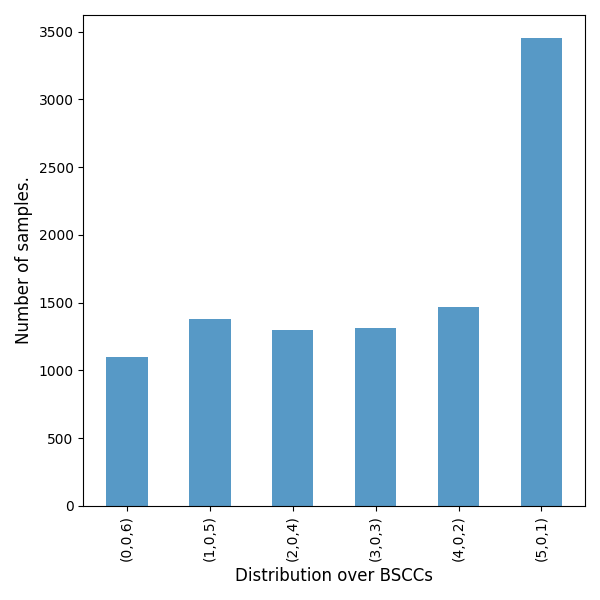
\includegraphics[width=\linewidth]{figures/sir510_data.png}
        \caption{SIR(5,1,0)}
    \end{subfigure}
    \hfill
    \begin{subfigure}{0.3\textwidth}
        \centering
        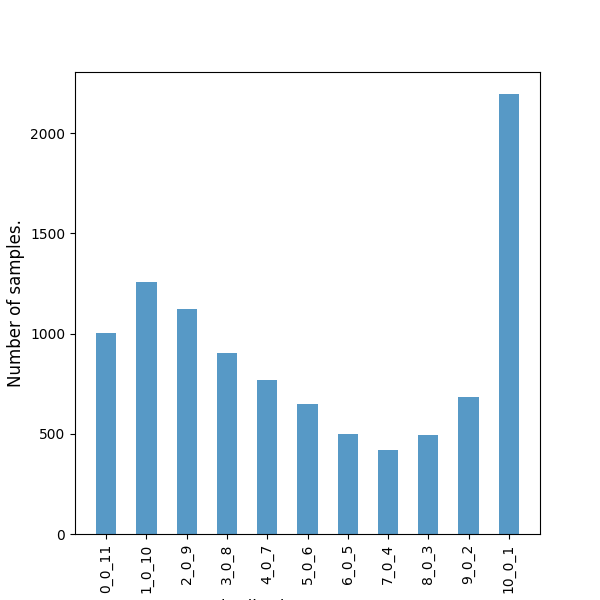
\includegraphics[width=\linewidth]{figures/sir1010_data.png}
        \caption{SIR(10,1,0)}
    \end{subfigure}
    \hfill
    \begin{subfigure}{0.3\textwidth}
        \centering
        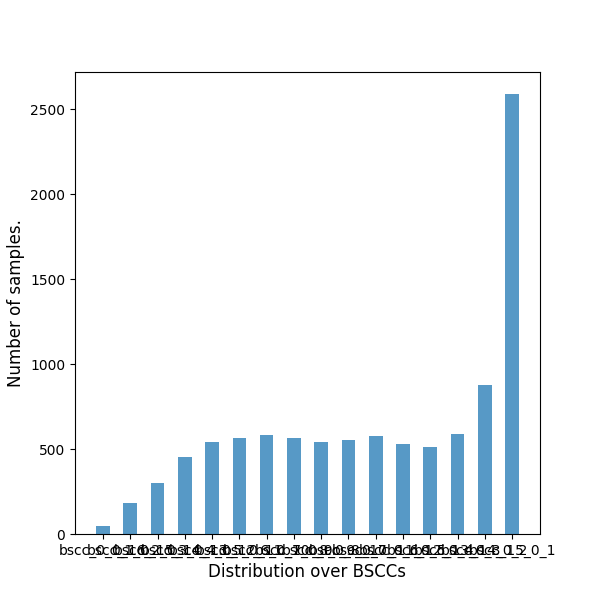
\includegraphics[width=\linewidth]{figures/sir1510_data.png}
        \caption{SIR(15,1,0)}
    \end{subfigure}
    \caption{Histograms of synthetic data $D_{obs}$.}
\end{figure}

We show examples of examples and counter-examples with simulations of CTMC. Using Gillespie
algorithm \cite{gillespie1976general} to simulate CTMC of selected $(\alpha, \beta)$, we show (i)
example of the property \textit{"the number of infected individuals does not exceed half of the
    population until the system is in its steady-state"} being satisfied, and (ii) its corresponding
counter-example.
\begin{figure}[H]
    \centering
    \begin{subfigure}{0.48\textwidth}
        \centering
        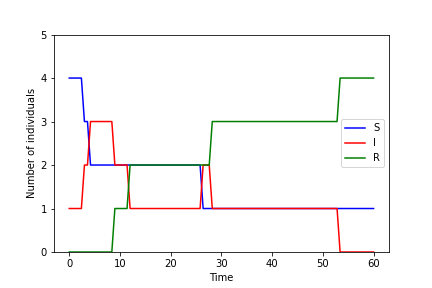
\includegraphics[width=\linewidth]{figures/sir_510_trace_1.png}
        \caption{Example with SIR(5,1,0)}
    \end{subfigure}
    \hfill
    \begin{subfigure}{0.48\textwidth}
        \centering
        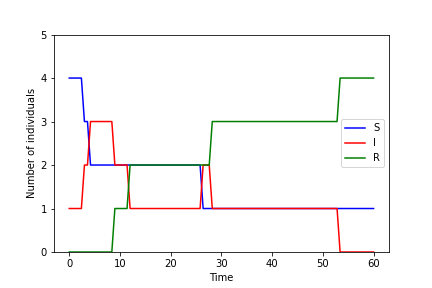
\includegraphics[width=\linewidth]{figures/sir_510_trace_1.png}
        \caption{Counter-example with SIR(5,1,0)}
    \end{subfigure}
    \caption{Example and counter-example on SIR(5,1,0) CTMC with $(\alpha, \beta)=(0.034055, 0.087735)$.}
\end{figure}
\begin{figure}[H]
    \centering
    \begin{subfigure}{0.48\textwidth}
        \centering
        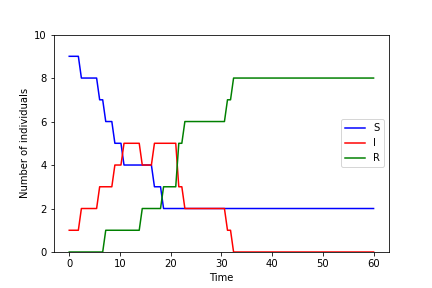
\includegraphics[width=\linewidth]{figures/sir_1010_trace_1.png}
        \caption{Example with SIR(10,1,0)}
    \end{subfigure}
    \hfill
    \begin{subfigure}{0.48\textwidth}
        \centering
        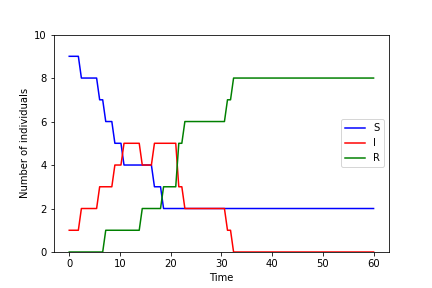
\includegraphics[width=\linewidth]{figures/sir_1010_trace_1.png}
        \caption{Counter-example with SIR(10,1,0)}
    \end{subfigure}
    \caption{Example and counter-example on SIR(10,1,0) CTMC with $(\alpha, \beta)=(0.025490, 0.069298)$.}
\end{figure}
\begin{figure}[H]
    \centering
    \begin{subfigure}{0.48\textwidth}
        \centering
        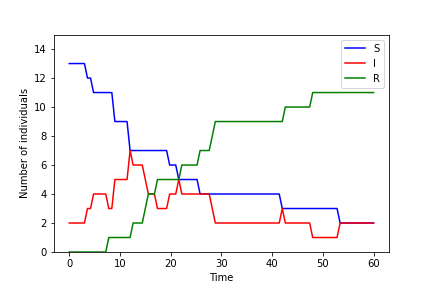
\includegraphics[width=\linewidth]{figures/sir_1510_trace_1.png}
        \caption{Example with SIR(15,1,0)}
    \end{subfigure}
    \hfill
    \begin{subfigure}{0.48\textwidth}
        \centering
        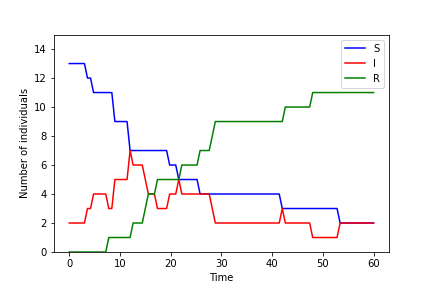
\includegraphics[width=\linewidth]{figures/sir_1510_trace_1.png}
        \caption{Counter-example with SIR(15,1,0)}
    \end{subfigure}
    \caption{Example and counter-example on SIR(15,1,0) CTMC with $(\alpha, \beta)=(0.011499, 0.062111)$.}
\end{figure}

\newpage
\subsubsection{Parameter synthesis result}
\noindent Parameter synthesis results for SIR(5,1,0) model:
\begin{table}[H]
    \begin{tabular}{|l|l|l|}
        \hline
        Method                                           & RF-SMC               & SMC-ABC-SMC          \\ \hline
        Estimated parameter $\hat{\theta}$               & (0.034055, 0.087734) & (0.034055, 0.087734) \\ \hline
        True parameter $\theta$                          & (0.025473, 0.067613) & (0.023077, 0.064812) \\ \hline
        L2 distance $\Vert \theta, \hat{\theta} \Vert_2$ & 0.021875             & 0.020120             \\ \hline
        $P(\mathcal{M}_{\hat{\theta}}\models\Phi)$       & 0.352182             & 0.347407             \\ \hline
    \end{tabular}
    \caption{Parameter estimation results for SIR(5,1,0) model.}
\end{table}

\begin{figure}[H]
    \centering
    \begin{subfigure}{0.48\textwidth}
        \centering
        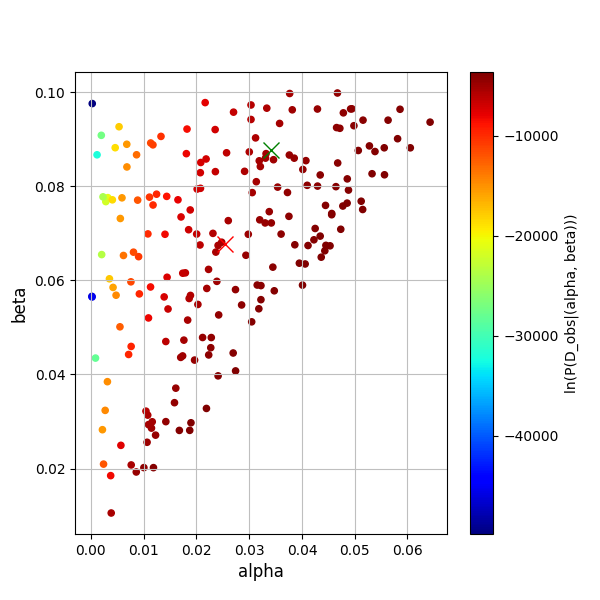
\includegraphics[width=\linewidth]{figures/sir510_rfsmc.png}
        \caption{Sampled particles using RF-SMC}
    \end{subfigure}
    \hfill
    \begin{subfigure}{0.48\textwidth}
        \centering
        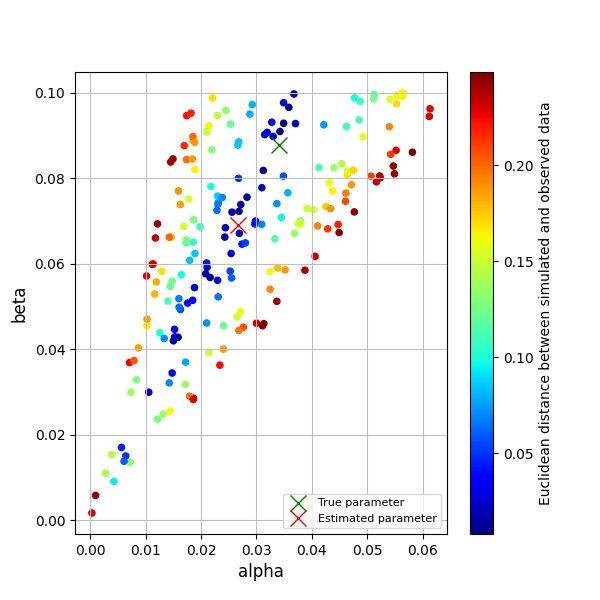
\includegraphics[width=\linewidth]{figures/sir510_abcsmc.png}
        \caption{Sampled particles using SMC-ABC-SMC}
    \end{subfigure}
    \caption{SIR(5,1,0) parameter synthesis results.}
\end{figure}

In the experiment with $SIR(5,1,0)$ model we observe that the rational-function-based method and
simulation-based method deliverresults without any significant difference.

\newpage
\noindent
Parameter synthesis results for SIR(10,1,0) model:
\begin{table}[H]
    \begin{tabular}{|l|l|l|}
        \hline
        Method                                           & RF-SMC               & SMC-ABC-SMC          \\ \hline
        Estimated parameter $\hat{\theta}$               & (0.014095, 0.066328) & (0.022552, 0.066416) \\ \hline
        True parameter $\theta$                          & (0.025490, 0.06930)  & (0.025490, 0.06930)  \\ \hline
        L2 distance $\Vert \theta, \hat{\theta} \Vert_2$ & 0.011776             & 0.004116             \\ \hline
        $P(\mathcal{M}_{\hat{\theta}}\models\Phi)$       & 0.363570             & 0.281154             \\ \hline
    \end{tabular}
    \caption{Parameter estimation results for SIR(10,1,0) model.}
\end{table}

\begin{figure}[H]
    \centering
    \begin{subfigure}{0.48\textwidth}
        \centering
        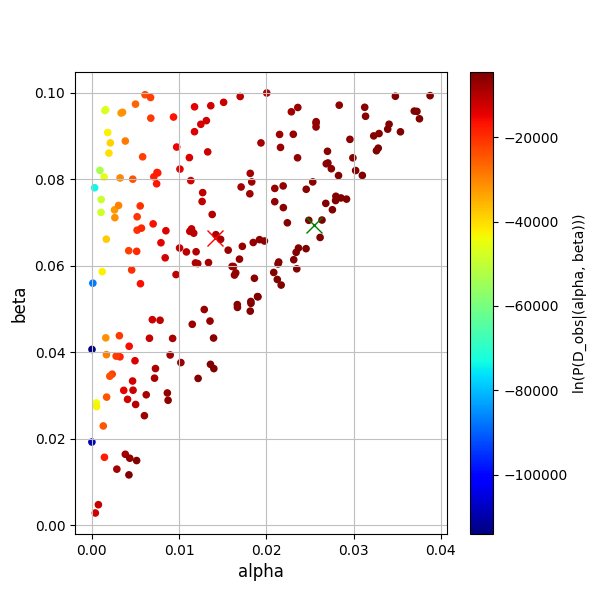
\includegraphics[width=\linewidth]{figures/sir1010_rfsmc.png}
        \caption{SIR(10,1,0), sampled particles using RF-SMC}
    \end{subfigure}
    \hfill
    \begin{subfigure}{0.48\textwidth}
        \centering
        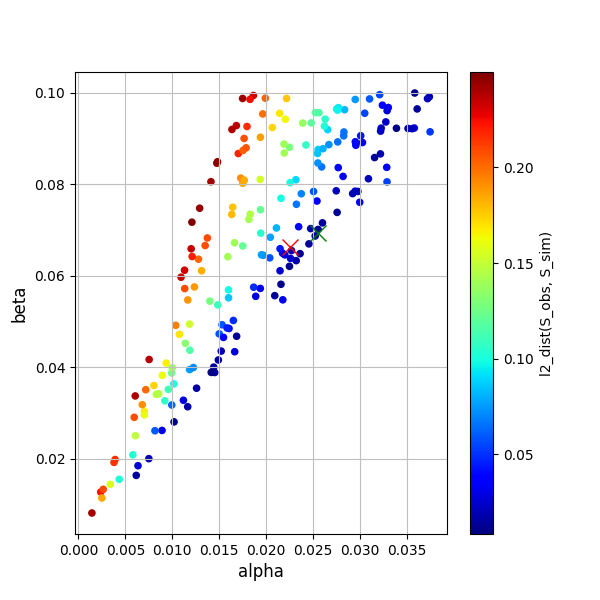
\includegraphics[width=\linewidth]{figures/sir1010_abcsmc.png}
        \caption{SIR(10,1,0), sampled particles using SMC-ABC-SMC}
    \end{subfigure}
    \caption{ parameter synthesis results.}
\end{figure}

In the experiment with $SIR(10,1,0)$ model we can see that the simulation-based method delivers a
closer estimation to true parameter. However, rational-function-based method gives an estimation
with higher satisfaction probability.

\newpage
\noindent Parameter synthesis results for SIR(15,1,0) model:
\begin{table}[H]
    \begin{tabular}{|l|l|l|}
        \hline
        Method                                           & RF-SMC               & SMC-ABC-SMC          \\ \hline
        Estimated parameter $\hat{\theta}$               & (0.012444, 0.065862) & (0.010022, 0.067230) \\ \hline
        True parameter $\theta$                          & (0.011499, 0.062111) & (0.011499, 0.062111) \\ \hline
        L2 distance $\Vert \theta, \hat{\theta} \Vert_2$ & 0.006545             & 0.005520             \\ \hline
        $P(\mathcal{M}_{\hat{\theta}}\models\Phi)$       & 0.366493             & 0.323579             \\ \hline
    \end{tabular}
    \caption{Parameter estimation results for SIR(15,1,0) model.}
\end{table}
In the experiment with $SIR(10,1,0)$ model we can see that the simulation-based method delivers a
slightly closer estimation to true parameter. Rational-function-based method gives an estimation
with higher satisfaction probability. However, overall, the estimations are comparable in terms of
accuracy an satisfaction probability

\begin{figure}[H]
    \centering
    \begin{subfigure}{0.48\textwidth}
        \centering
        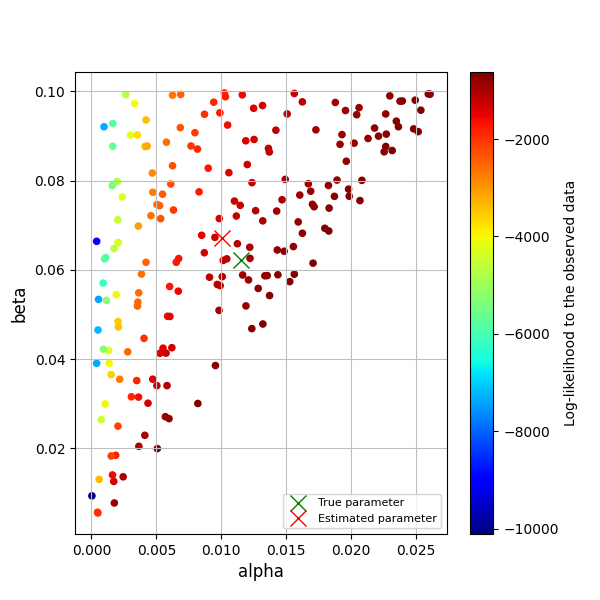
\includegraphics[width=\linewidth]{figures/sir1510_rfsmc.png}
        \caption{Sampled particles using RF-SMC}
    \end{subfigure}
    \hfill
    \begin{subfigure}{0.48\textwidth}
        \centering
        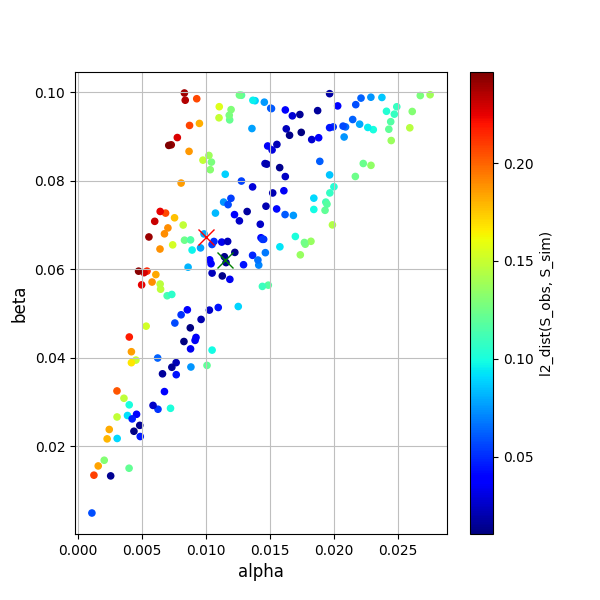
\includegraphics[width=\linewidth]{figures/sir1510_abcsmc.png}
        \caption{Sampled particles using SMC-ABC-SMC}
    \end{subfigure}
    \caption{SIR(15,1,0) parameter synthesis results.}
\end{figure}

\newpage
\noindent We study the behavior of both frameworks when less data is available. Instead of using
synthetic data of $10000$ samples, we use $200$ samples as observed data for parameter synthesis and
estimation. We also introduce uncertainty by merging BSCCs into 2 bins: one consists of BSCCs with
more than half of the population remain uninfected, and the other consists of all BSCCs left. This
adjustment to the DTMC is made by merging BSCCs into a single BSCC. \\
We perform the experiment on SIR(15,1,0) with only two BSCCs: (i) BSCCs with $S \leq 8$, and (ii)
BSCC with $S > 8$. The results are then summarized into the following table:

\begin{table}[H]
    \begin{tabular}{|l|l|l|}
        \hline
        Method                                           & RF-SMC                   & SMC-ABC-SMC          \\ \hline
        Estimated parameter $\hat{\theta}$               & (0.00945054, 0.06634182) & (0.016698, 0.081153) \\ \hline
        True parameter $\theta$                          & (0.011499, 0.062111)     & (0.011499, 0.062111) \\ \hline
        L2 distance $\Vert \theta, \hat{\theta} \Vert_2$ & 0.004701                 & 0.019740             \\ \hline
        \begin{tabular}[c]{@{}l@{}}Satisfaction property\\ $P(\mathcal{M}_{\hat{\theta}}\models\Phi)$\end{tabular}                       & 0.374375                 & 0.306351             \\ \hline
    \end{tabular}
    \caption{Parameter estimation results for SIR(15,1,0) model with merged BSCC.}
\end{table}

\begin{figure}[H]
    \centering
    \begin{subfigure}{0.48\textwidth}
        \centering
        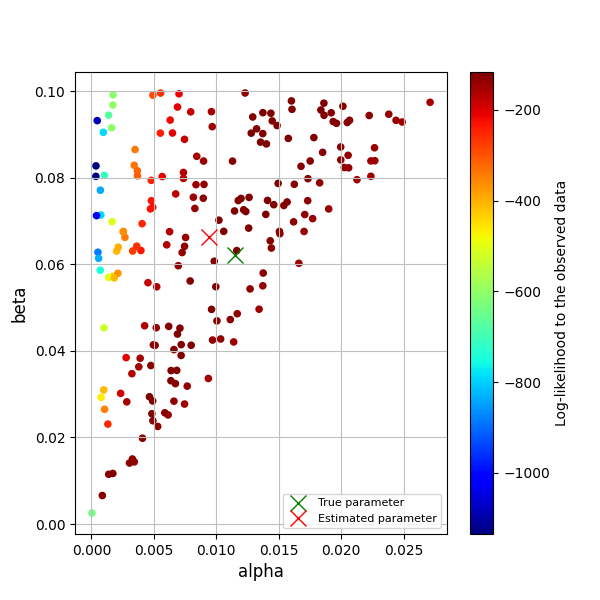
\includegraphics[width=\linewidth]{figures/sir1510_merged_bscc_rfsmc.png}
        \caption{Sampled particles using RF-SMC}
    \end{subfigure}
    \hfill
    \begin{subfigure}{0.48\textwidth}
        \centering
        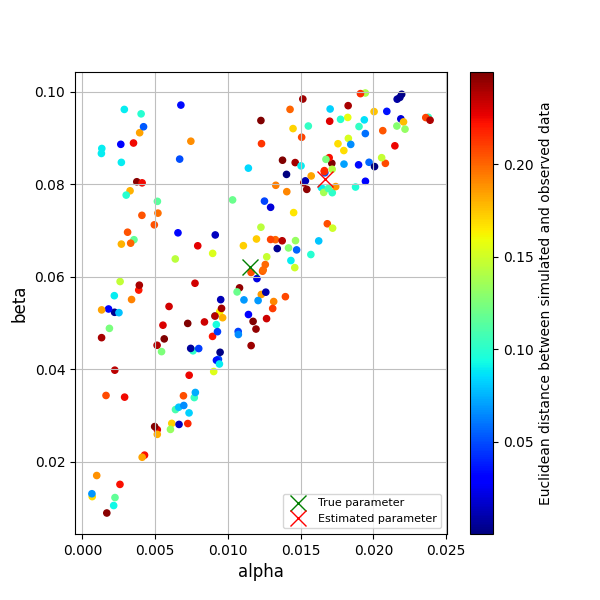
\includegraphics[width=\linewidth]{figures/sir1510_merged_bscc_abcsmc.png}
        \caption{Sampled particles using SMC-ABC-SMC}
    \end{subfigure}
    \caption{Parameter synthesis results for SIR(15,1,0) model with merged BSCC.}
\end{figure}

Unlike experiments with SIR(15,1,0) without merging BSCCs, the experiment with merged BSCCs and
simulation-based framework shows no general pattern of distance among satisfying parameter values.
It is hypothetically because of the noisy data that leads to a non-converging evaluation of distance
between simulated data and observed data \cite{sisson2007sequential}. A proposed way to solve the
problem is to use a decreasing threshold scheme, in which $\epsilon$ decreases after each
perturbation. We experiment again with the distance threshold decreases by a factor $0.95$ after
each perturbation round. The result is then visualized:
\begin{figure}[H]
    \centering
    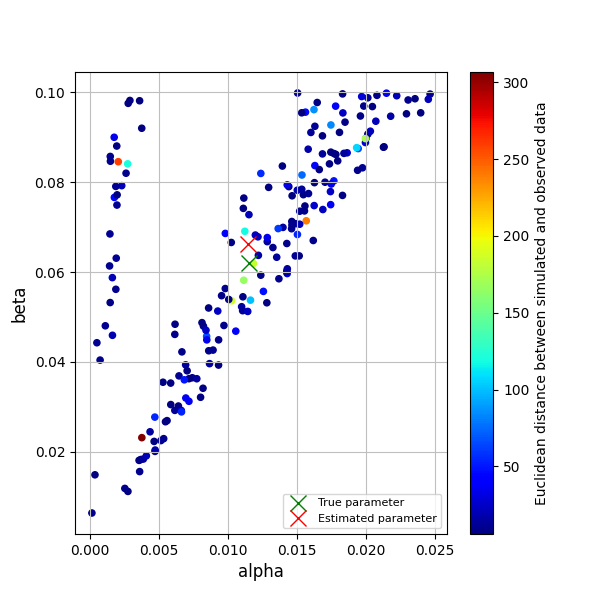
\includegraphics[width=0.5\linewidth]{figures/sir1510_merged_bscc_abcsmc_mod.png}
    \caption{Parameter synthesis results for SIR(15,1,0) model with merged BSCC and decreasing distance threshold.}
\end{figure}
The estimated parameter is $(0.01148671, 0.06624936)$, closer to the true parameter (Euclidean
distance is $0.004138$), and the satisfaction probability $P(\mathcal{M}_{\alpha,\beta}) = 0.336849$.

\subsection{Performance}
To measure the performance of RF-SMC and SMC-ABC-SMC, we measure the physical runtime to finish
\textit{(total runtime)} and the average physical run time of one perturbation kernel
\textit{(average perturbation runtime)}.

\begin{table}[H]
    \centering
    \begin{tabular}{|l|l|l|}
        \hline
        Method                     & RF-SMC & SMC-ABC-SMC \\ \hline
        Total runtime (minutes)    & 5.917  & 68.783      \\ \hline
        \begin{tabular}[c]{@{}l@{}}Average perturbation\\ runtime (minutes)\end{tabular} & 0.312  & 3.614       \\ \hline
    \end{tabular}
    \caption{Physical runtime on SIR(5,1,0) model.}
\end{table}
\begin{table}[H]
    \centering
    \begin{tabular}{|l|l|l|}
        \hline
        Method                     & RF-SMC & SMC-ABC-SMC \\ \hline
        Total runtime (minutes)    & 29.517 & 352.083     \\ \hline
        \begin{tabular}[c]{@{}l@{}}Average perturbation\\ runtime (minutes)\end{tabular} & 1.553  & 18.518      \\ \hline
    \end{tabular}
    \caption{Physical runtime on SIR(10,1,0) model.}
\end{table}
\begin{table}[H]
    \centering
    \begin{tabular}{|l|l|l|}
        \hline
        Method                     & RF-SMC   & SMC-ABC-SMC \\ \hline
        Total runtime (minutes)    & 3976.117 & 581.833     \\ \hline
        \begin{tabular}[c]{@{}l@{}}Average perturbation\\ runtime (minutes)\end{tabular} & 209.237  & 30.592      \\ \hline
    \end{tabular}
    \caption{Physical runtime on SIR(15,1,0) model.}
\end{table}
\begin{figure}[H]
    \centering
    \begin{subfigure}{0.48\textwidth}
        \centering
        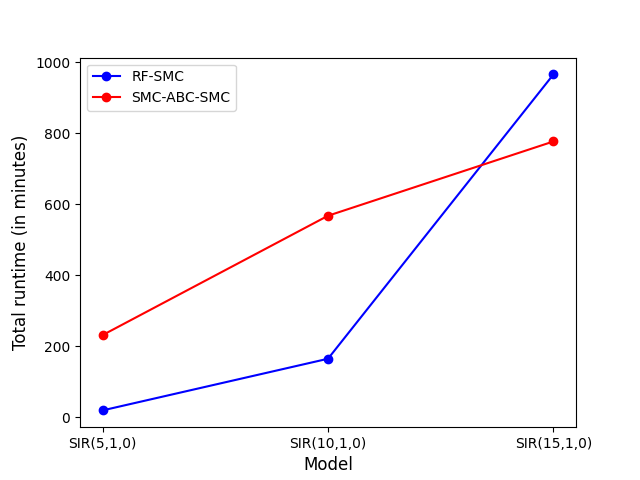
\includegraphics[width=\linewidth]{figures/sir_runtime_total.png}
        \caption{Total runtime}
    \end{subfigure}
    \hfill
    \begin{subfigure}{0.48\textwidth}
        \centering
        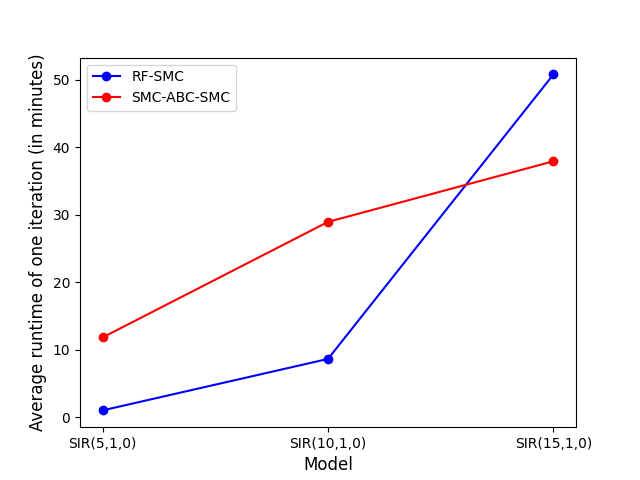
\includegraphics[width=\linewidth]{figures/sir_runtime_avg.png}
        \caption{Average perturbation runtime}
    \end{subfigure}
    \caption{Physical runtime on SIR models of different population sizes.}
\end{figure}

\subsection{Discussion}
As the performance statistics show, as the state-space of a parametric DTMC grows, the
rational-function-based method becomes more expensive in computational cost than the
simulation-based method. However, as the last experiment shows, Approximate Bayesian Computation
does not accurately approximate the posterior when less data is provided. However, we also shown
that combining with a decreasing distance threshold to approximate the likelihood more precisely,
SMC-ABC-SMC shows a comparable accuracy to rational-function-based RF-SMC. Therefore, experiments
with SIR models suggest that the simulation-based method is superior to rational-function-based
method.



